\documentclass{beamer}
\usepackage[utf8]{inputenc}
\usepackage{palatino} % use palatino as the default font
\usepackage{listings}
\usetheme{Warsaw}

\lstset{ %
language=Octave,                % choose the language of the code
basicstyle=\tiny,       	% the size of the fonts that are used for the code
numbers=left,                   % where to put the line-numbers
numberstyle=\tiny,      	% the size of the fonts that are used for the line-numbers
stepnumber=1,                   % the step between two line-numbers. If it's 1 each line 
                                % will be numbered
numbersep=10pt,                  % how far the line-numbers are from the code
backgroundcolor=\color{white},  % choose the background color. You must add \usepackage{color}
showspaces=false,               % show spaces adding particular underscores
showstringspaces=false,         % underline spaces within strings
showtabs=false,                 % show tabs within strings adding particular underscores
frame=single,	                % adds a frame around the code
tabsize=2,	                % sets default tabsize to 2 spaces
captionpos=b,                   % sets the caption-position to bottom
breaklines=true,                % sets automatic line breaking
breakatwhitespace=false,        % sets if automatic breaks should only happen at whitespace
title=\tiny\lstname,            % show the filename of files included with \lstinputlisting;
                                % also try caption instead of title
escapeinside={\%*}{*)},         % if you want to add a comment within your code
morekeywords={*,...},           % if you want to add more keywords to the set
frameround=fttt,
}

\title{Analysing differences in tree-structured data by Visual Analytics}
\author{Johannes Lichtenberger}\institute{Distributed Systems Group}

\begin{document}

\begin{frame}
\titlepage
\end{frame}

\begin{frame}
\frametitle{Motivation - State of the art}
\begin{center}
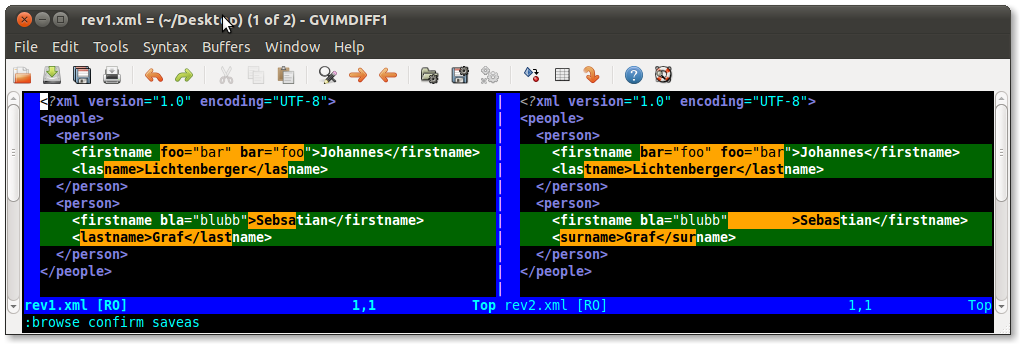
\includegraphics[width=4.0in]{images/gvimdiff.png}
\end{center}
\end{frame}

\begin{frame}
\frametitle{SunburstView}
\begin{center}
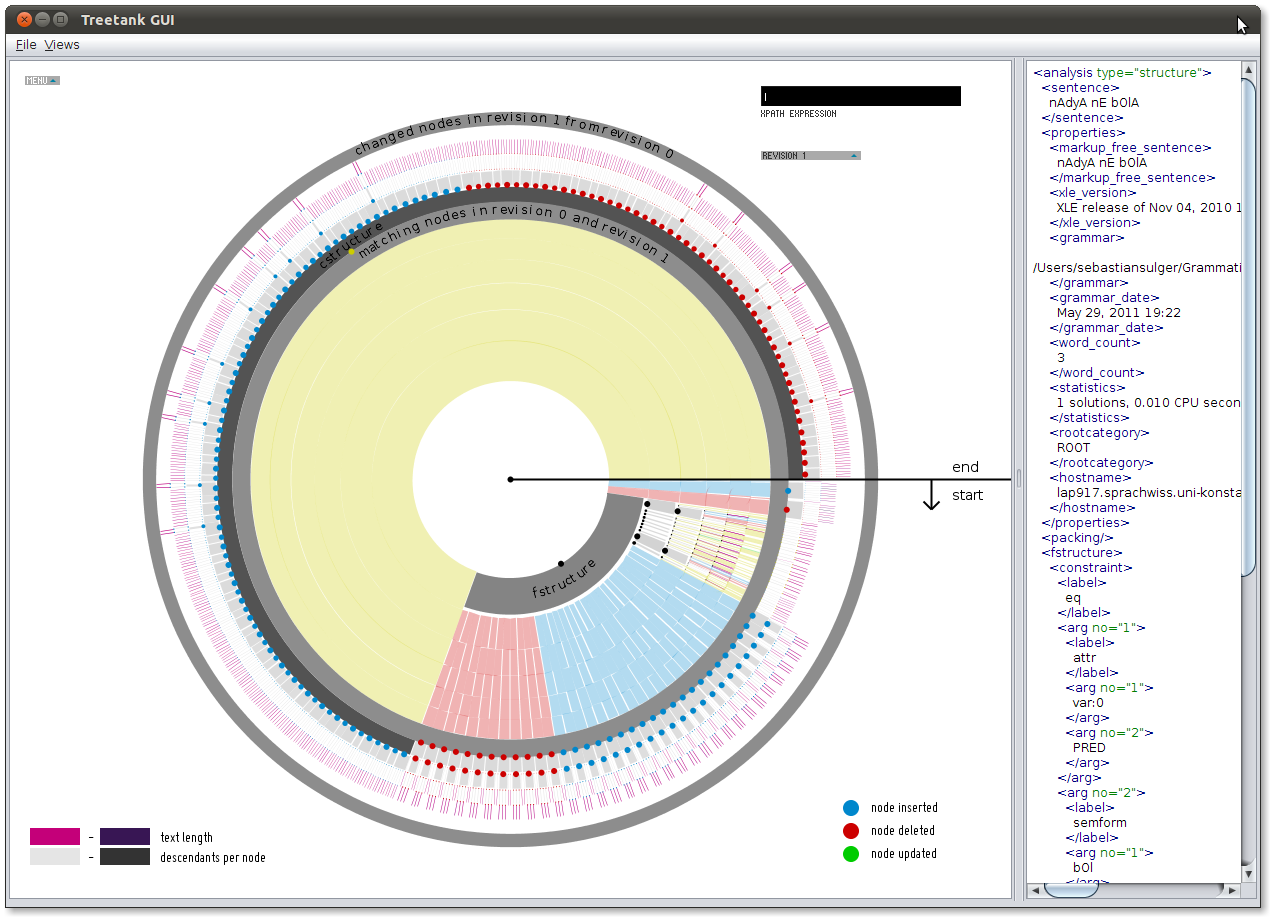
\includegraphics[width=3.5in]{images/treetank-gui.png}
\end{center}
\end{frame}

\begin{frame}
\frametitle{SmallMultiplesView}
\begin{center}
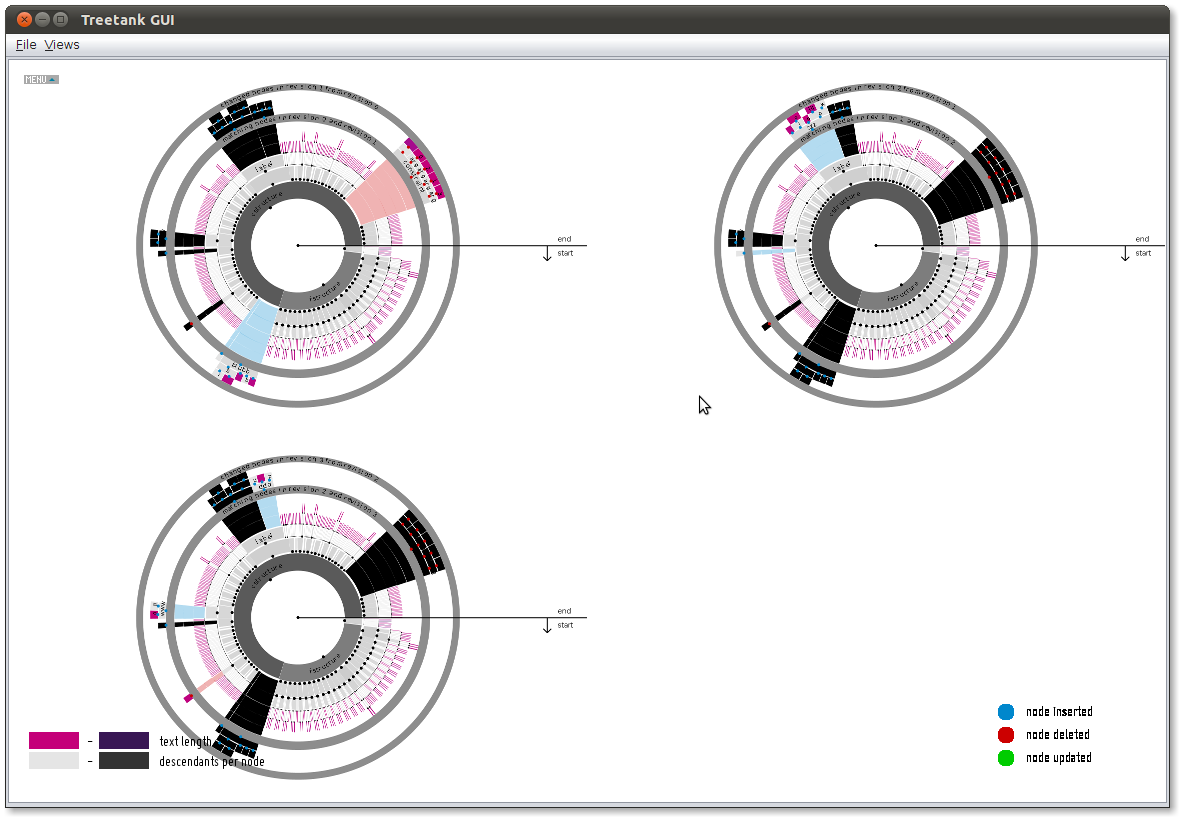
\includegraphics[width=3.5in]{images/treetank-gui-smallmultiples.png}
\end{center}
\end{frame}

%\begin{frame}
%\frametitle{Visualization Challenges}
%Visualization challenges (single view):

%\begin{enumerate}
%\item items require startAngle, extension, descendantCount, modificationCount, kind of diff
%\item agglomeration
%\item pruning
%\item provide the enlargement of changed nodes
%\item reducing maxDepth in inner circle if nodes at maxDepth have been changed
%\item descendant-or-self count per node including deleted nodes
%\end{enumerate}
%\end{frame}

%\begin{frame}
%\frametitle{Challenges - Continued}
%Small Multiples:

%\begin{enumerate}
%\item adding further abstraction
%\item multithreading -- lock firing of changes in the model
%\item multithreading -- requires sorting of offscreen buffers
%\item greyout
%\end{enumerate}
%\end{frame}

\begin{frame}
\frametitle{Visualization Challenges - SunburstDiffAxis}
\begin{center}
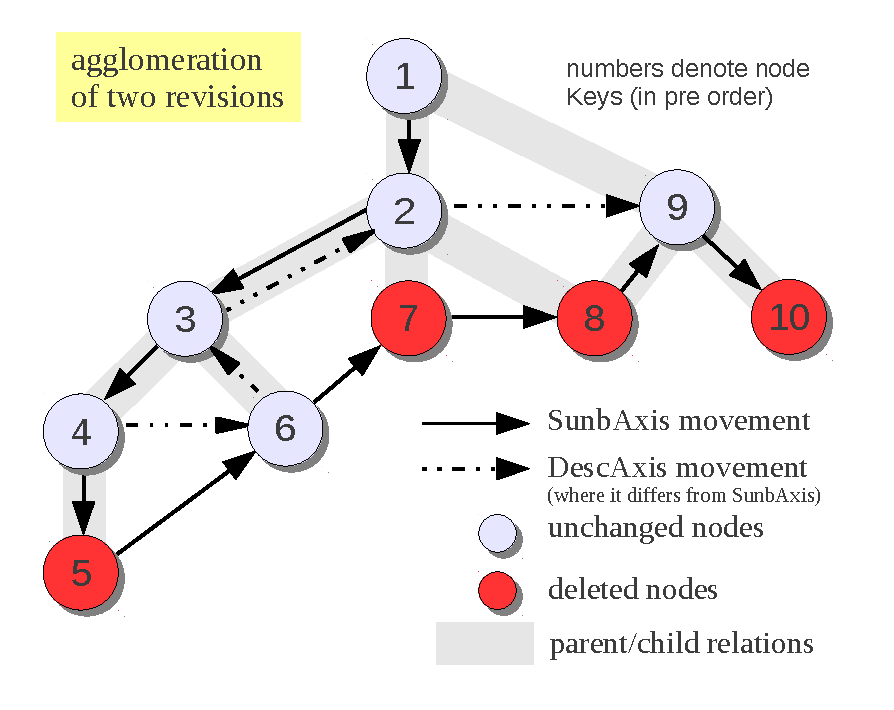
\includegraphics[width=4.0in]{images/tree-axis.pdf}
\end{center}
\end{frame}

\begin{frame}
\frametitle{Demo}
Demo...
\end{frame}

\begin{frame}
\frametitle{Future work}
Next step:

\begin{itemize}
\item Specialized XPath-axis to further enhance and support the analytical part of "Visual Analytics"
\end{itemize}

Possible additional work:

\begin{itemize}
\item Detection of moves in the ID-based diff algorithm
\item Visualization of moves
\end{itemize}
\end{frame}

\begin{frame}
\frametitle{Appendix}
\begin{block}{\centering Analytical part so far}
\centering A highlevel overview.
\end{block}
\end{frame}

\begin{frame}
\frametitle{Analytical Part - Overview}
\begin{center}
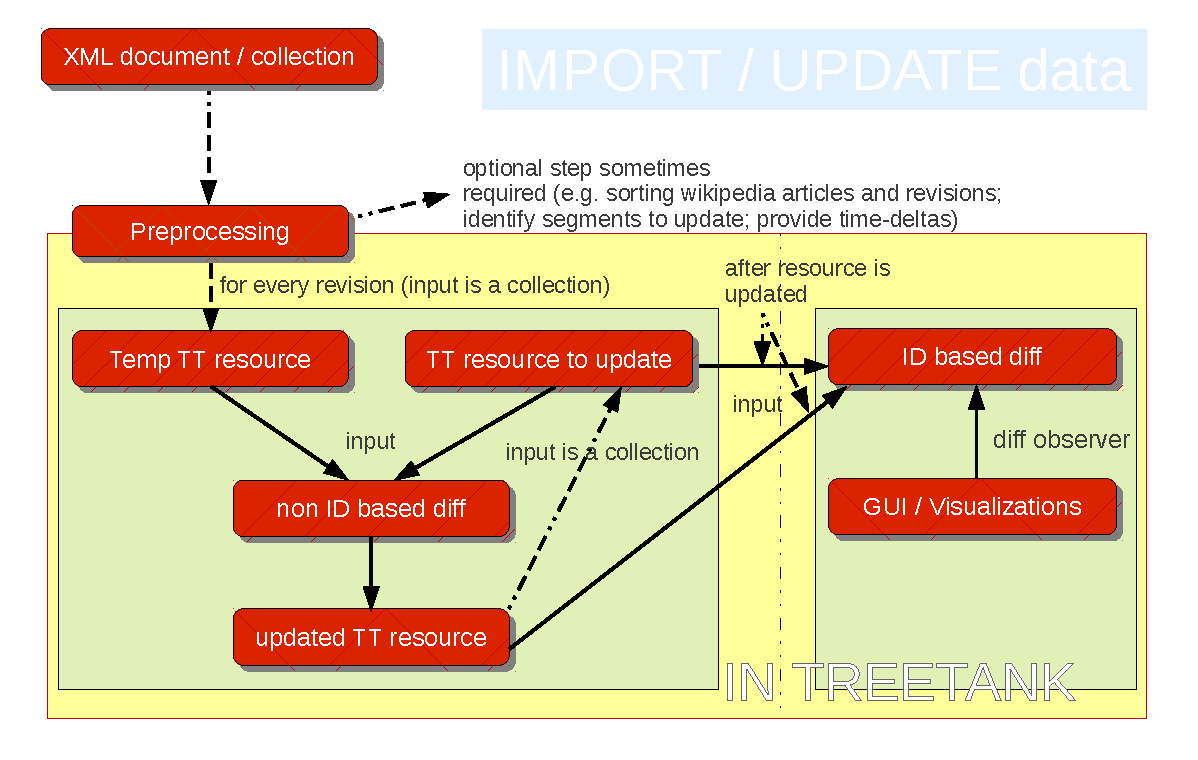
\includegraphics[width=4.0in]{images/importdata.pdf}
\end{center}
\end{frame}

\begin{frame}
\frametitle{Analytical Part - ID-less diff matching (from the paper "Change Detection in Hierarichally Structured Data")}
\begin{center}
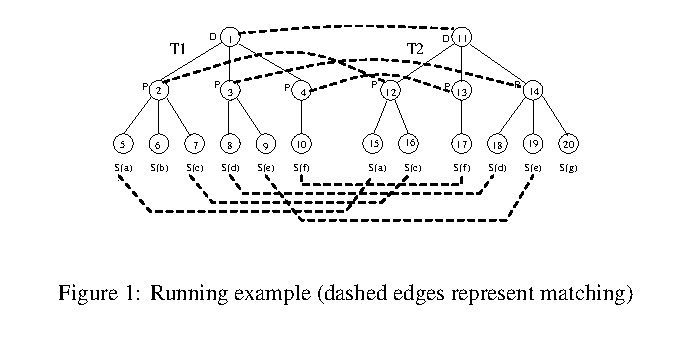
\includegraphics[width=4.5in]{images/matching.pdf}
\end{center}
\end{frame}

\end{document}
